\documentclass{article}
\usepackage{tikz}
\usetikzlibrary{calc}

\begin{document}

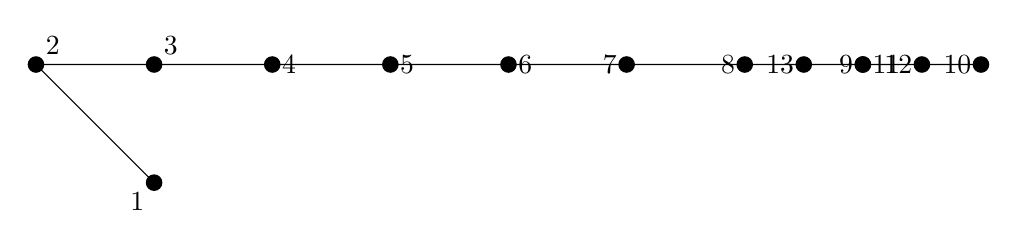
\begin{tikzpicture}[scale=1.5]
    % Define the coordinates of the vertices
    \coordinate (A) at (0,0);
    \coordinate (B) at (-1,1);
    \coordinate (C) at (0,1);
    \coordinate (D) at (1,1);
    \coordinate (E) at (2,1);
    \coordinate (F) at (3,1);
    \coordinate (G) at (4,1);
    \coordinate (H) at (5,1);
    \coordinate (I) at (6,1);
    \coordinate (J) at (7,1);

    % Draw the edges of the graph
    \draw[-] (A) -- (B) -- (C) -- (D) -- (E) -- (F) -- (G) -- (H) -- (I) -- (J);
    \draw[-] (B) -- (D);
    \draw[-] (C) -- (F);
    \draw[-] (D) -- (G);
    \draw[-] (E) -- (H);
    \draw[-] (F) -- (I);
    \draw[-] (G) -- (J);
    \draw[-] (J) -- (H);
    \draw[-] (I) -- (G);
    \draw[-] (H) -- (F);
    \draw[-] (G) -- (D);
    \draw[-] (F) -- (C);
    \draw[-] (E) -- (B);
    
    % Label the vertices
    \fill (A) circle (2pt) node[anchor=north east] {$1$};
    \fill (B) circle (2pt) node[anchor=south west] {$2$};
    \fill (C) circle (2pt) node[anchor=south west] {$3$};
    \fill (D) circle (2pt) node[anchor=west] {$4$};
    \fill (E) circle (2pt) node[anchor=west] {$5$};
    \fill (F) circle (2pt) node[anchor=west] {$6$};
    \fill (G) circle (2pt) node[anchor=east] {$7$};
    \fill (H) circle (2pt) node[anchor=east] {$8$};
    \fill (I) circle (2pt) node[anchor=east] {$9$};
    \fill (J) circle (2pt) node[anchor=east] {$10$};
    \fill ($(H)!0.5!(J)$) circle (2pt) node[anchor=west] {$11$};
    \fill ($(J)!0.5!(I)$) circle (2pt) node[anchor=east] {$12$};
    \fill ($(I)!0.5!(H)$) circle (2pt) node[anchor=east] {$13$};
\end{tikzpicture}

\small\sf An outerplanar graph without degree-1 vertices. The triangle $(5,7,9)$ is the only internal cycle, while $(1,2,3)$, $(3,4,5,6,7,8,9,10)$, and $(11,12,13)$ are outer-cycles. A possible cyclic-order is $(1,2,3,4,5,6,7,8,9,10,11,12,13)$.

\end{document}